\documentclass[11pt]{article}
\usepackage{authblk}
\usepackage[hidelinks]{hyperref}
\usepackage{style/acl2016}

\usepackage{times}
\usepackage{url}
\usepackage{latexsym}
\usepackage{amsmath}

%\usepackage{apacite}
\usepackage{graphicx}
\usepackage{epstopdf}
\usepackage{amsmath}
\usepackage{amssymb}
\usepackage{enumerate}
\usepackage{mdwlist}
\usepackage{nomencl}
%\usepackage[table]{xcolor}
\usepackage{CJKutf8}
\usepackage[utf8]{inputenc}

\usepackage{newunicodechar}
\def\aclpaperid{55}
\aclfinalcopy
\DeclareUnicodeCharacter{FFFD}{?????}
% Comment
\usepackage[usenames]{color}

%\newif\ifcomment\commenttrue
\newif\ifcomment\commentfalse

\setlength\titlebox{6cm}

% Preamble file contains handy macros and most packages you might want to use.
% At the start are packages that conflict with various styles.  Don't add them
% in!  Just put it in your main TeX file instead.

% Do not put either of these (subfigure or subfloat) into the preamble
% - they clash.  Use them in the final LaTeX document
% \usepackage{subfigure}
% \suepackage{subfloat}

% Do not use times in the preamble!  It just causes problems with some
% publication chairs (e.g., ICML 2013).  If you want it, put it in your own
% document.
% \usepackage{times}


% Breaks ACM-SIG style
% \usepackage{titlesec}
% \usepackage{amsthm}
% \usepackage{nomencl}

% comment out the following line, as it conflicts with aistats2012.sty
%\usepackage{caption}

% This is required by NSF.  Do not remove; if it conflicts with
% another package, fix that problem without removing this from
% Preamble.
% Unless for AAAI ... this needs a new bibfile that plays well with hyperref.
%\usepackage[a-1b]{pdfx}

% Below should be safe
\usepackage{framed}
\usepackage{mdwlist}
\usepackage{latexsym}
\usepackage{colortbl}
\usepackage{xcolor}
\usepackage{nicefrac}
\usepackage{booktabs}
\usepackage{amsfonts}
\usepackage[T1]{fontenc}
\usepackage{bold-extra}
\usepackage{amsmath}
\usepackage{amssymb}
\usepackage{bm}
\usepackage{graphicx}
\usepackage{mathtools}
\usepackage{microtype}
\usepackage{multirow}
\usepackage{multicol}
% Don't use hyperref or url, as it can screw up AAAI / ICML formatting
%\usepackage{url}
\usepackage{latexsym,comment}
\usepackage[normalem]{ulem}

\newcommand{\breakalign}{\right. \nonumber \\ & \left. \hspace{2cm}}



\newcommand{\feat}[1]{{\small \texttt{#1}}}
\newcommand{\act}[1]{{\small \texttt{#1}}}
\newcommand{\ngram}[0]{$n$-gram}
\newcommand{\topic}[1]{\underline{#1}}
\newcommand{\gem}[1]{\mbox{\textsc{gem}}}
\newcommand{\abr}[1]{\textsc{#1}}
\newcommand{\camelabr}[2]{{\small #1}{\textsc{#2}}}
\newcommand{\abrcamel}[2]{{\textsc #1}{\small{#2}}}
\newcommand{\grammar}[1]{{\color{red} #1}}
\newcommand{\explain}[2]{\underbrace{#2}_{\mbox{\footnotesize{#1}}}}
\newcommand{\dir}[1]{\mbox{Dir}(#1)}
\newcommand{\bet}[1]{\mbox{Beta}(#1)}
\newcommand{\py}[1]{\mbox{\textsc{py}}(#1)}
\newcommand{\td}[2]{\mbox{\textsc{TreeDist}}_{#1} \left( #2 \right)}
\newcommand{\yield}[1]{\mbox{\textsc{Yield}} \left( #1 \right)}
\newcommand{\mult}[1]{\mbox{Mult}( #1)}
\newcommand{\wn}{\textsc{WordNet}}
\newcommand{\twentynews}{\textsc{20news}}
\newcommand{\g}{\, | \,}
\newcommand{\Gam}[1]{\Gamma \left( \textstyle #1 \right)}
\newcommand{\LG}[1]{\log \Gamma \left( \textstyle #1 \right)}
\newcommand{\Pois}[1]{\mbox{Poisson}(#1)}
\newcommand{\pcfg}[3]{#1_{#2 \rightarrow #3}}
\newcommand{\grule}[2]{#1 \rightarrow #2}
\newcommand{\kl}[2]{D_{\mbox{\textsc{KL}}} \left( #1 \,||\, #2 \right)}

\newcommand{\digambig}[1]{\Psi \left( #1 \right) }
\newcommand{\digam}[1]{\Psi \left( \textstyle #1 \right) }
\newcommand{\ddigam}[1]{\Psi' \left( \textstyle #1 \right) }


\renewenvironment{quote}
               {\list{}{\rightmargin\leftmargin}%
                \item\relax\small\ignorespaces}
               {\unskip\unskip\endlist}

\DeclareMathOperator*{\argmax}{arg\,max}
\DeclareMathOperator*{\argmin}{arg\,min}
\newcommand{\bmat}[1]{\text{\textbf{#1}}}
\newcommand{\bvec}[1]{\boldsymbol{#1}}

%\newcommand{\email}[1]{ {\small \href{mailto://#1}{\texttt{#1} }  }}
\newcommand{\emaillink}[1]{ {\small \href{mailto://#1}{\texttt{#1}}}}
\newcommand{\smallemaillink}[2]{ {\small \href{mailto://#2}{\texttt{#1}}}}

% JBG: Consider renaming from \ch to \zh because of conflict when adding Cyrillic
\newcommand{\ch}[1]{\begin{CJK*}{UTF8}{gbsn}#1\end{CJK*}}

\newcommand{\e}[2]{\mathbb{E}_{#1}\left[ #2 \right] }
\newcommand{\h}[2]{\mathbb{H}_{#1}\left[ #2 \right] }
\newcommand{\ind}[1]{\mathds{1}\left[ #1 \right] }
\newcommand{\ex}[1]{\mbox{exp}\left\{ #1\right\} }
\newcommand{\D}[2]{\frac{\partial #1}{\partial #2}}
\newcommand{\elbo}{\mathcal{L}}

\newcommand{\hidetext}[1]{}
\newcommand{\ignore}[1]{}

\newcommand{\todo}[1]{\textcolor{red}{{\bf TODO: #1}}}

\ifcomment
\newcommand{\pinaforecomment}[3]{\colorbox{#1}{\parbox{.8\linewidth}{#2: #3}}}
\else
\newcommand{\pinaforecomment}[3]{}
\fi

\newcommand{\jbgcomment}[1]{\pinaforecomment{red}{JBG}{#1}}
\newcommand{\mjpcomment}[1]{\pinaforecomment{blue}{MJP}{#1}}
\newcommand{\czcomment}[1]{\pinaforecomment{orange}{chen}{#1}}
\newcommand{\ffcomment}[1]{\pinaforecomment{red}{FF}{#1}}
\newcommand{\fpcomment}[1]{\pinaforecomment{green}{FP}{#1}}
\newcommand{\yhcomment}[1]{\pinaforecomment{green}{YH}{#1}}
\newcommand{\hhecomment}[1]{\pinaforecomment{blue}{HH}{#1}}
\newcommand{\tncomment}[1]{\pinaforecomment{blue}{TN}{#1}}
\newcommand{\mnicomment}[1]{\pinaforecomment{green}{Mohit}{#1}}
\newcommand{\prcomment}[1]{\pinaforecomment{lightblue}{Pedro}{#1}}
\newcommand{\fscomment}[1]{\pinaforecomment{orange}{Shi}{#1}}
\newcommand{\vmcomment}[1]{\pinaforecomment{yellow}{Varun}{#1}}
\newcommand{\rscomment}[1]{\pinaforecomment{yellow}{Richard}{#1}}
\newcommand{\jszcomment}[1]{\pinaforecomment{green}{JSG}{#1}}
\newcommand{\ascomment}[1]{\pinaforecomment{blue}{AS}{#1}}
\newcommand{\vecomment}[1]{\pinaforecomment{blue}{VE}{#1}}
\newcommand{\halcomment}[1]{\pinaforecomment{magenta!20}{Hal}{#1}}
\newcommand{\kgcomment}[1]{\pinaforecomment{blue}{Kim}{#1}}
\newcommand{\vancomment}[1]{\pinaforecomment{green}{VAN}{#1}}
\newcommand{\thangcomment}[1]{\pinaforecomment{green}{Thang}{#1}}
\newcommand{\alvincomment}[1]{\pinaforecomment{cyan}{Alvin}{#1}}
\newcommand{\reviewercomment}[1]{\pinaforecomment{blue}{Reviewer}{#1}}
\newcommand{\brscomment}[1]{\pinaforecomment{blue}{BRS}{#1}}
\newcommand{\psrcomment}[1]{\pinaforecomment{yellow}{PSR}{#1}}
\newcommand{\zkcomment}[1]{\pinaforecomment{cyan}{ZK}{#1}}
\newcommand{\swcomment}[1]{\pinaforecomment{yellow}{SW}{#1}}
\newcommand{\shaycomment}[1]{\pinaforecomment{yellow}{SBC}{#1}}
\newcommand{\jlundcomment}[1]{\pinaforecomment{cyan}{J}{#1}}
\newcommand{\kdscomment}[1]{\pinaforecomment{ceil}{KDS}{#1}}
\newcommand{\lkfcomment}[1]{\pinaforecomment{yellow}{LF}{#1}}
\newcommand{\yfcomment}[1]{\pinaforecomment{brown}{YF}{#1}}
\newcommand{\ewcomment}[1]{\pinaforecomment{lightblue}{Eric}{#1}}
\newcommand{\pgcomment}[1]{\pinaforecomment{cyan}{Pranav}{#1}}
\newcommand{\bencomment}[1]{\pinaforecomment{lightblue}{Ben}{#1}}

\newcommand{\smalltt}[1]{ {\tt \small #1 }}
\newcommand{\smallurl}[1]{ \begin{tiny}\url{#1}\end{tiny}}
%\newcommand{\smallurl}[1]{ \begin{tiny} HIDDEN \end{tiny}}
\newenvironment{compactenum}{ \begin{enumerate*} \small }{ \end{enumerate*} }

\definecolor{lightblue}{HTML}{3cc7ea}
\definecolor{CUgold}{HTML}{CFB87C}
\definecolor{grey}{rgb}{0.95,0.95,0.95}
\definecolor{ceil}{rgb}{0.57, 0.63, 0.81}
\definecolor{UMDred}{HTML}{ed1c24}
\definecolor{UMDyellow}{HTML}{ffc20e}

% Datasets / Models

\newcommand{\qb}[0]{Quizbowl}
\newcommand{\qa}[0]{\abr{qa}}
\newcommand{\triviaqa}{\camelabr{Trivia}{qa}}
\newcommand{\searchqa}{\camelabr{Search}{qa}}
\newcommand{\qblink}{\abrcamel{qb}{Link}}
\newcommand{\qanta}{\textsc{qanta}}
\newcommand{\muse}{\textsc{muse}}
\newcommand{\squad}{\textsc{sq}{\small u}\textsc{ad}}
\newcommand{\fever}{\abr{fever}}
\newcommand{\quac}{\textsc{q}{\small u}\textsc{ac}}
\newcommand{\elmo}{\textsc{elm}{\small o}}
\newcommand{\fone}{$F_1$}
\newcommand{\jeopardy}{\textit{Jeopardy!}}

\DeclareMathOperator*{\argmax}{arg\,max}

\newcommand{\listsep}[0]{ \setlength{\parskip}{-0.2cm}}

% gloss
\newcommand{\gl}[2]{%
\leavevmode\vtop{\hbox{#1}%
\hbox{#2\lower1.4ex\rlap{}}}}

\title{Incremental Prediction of Sentence-final Verbs: Humans versus Machines}

\author{
  Alvin C. {Grissom II}$^{1}$, Naho Orita$^{2}$, and Jordan {Boyd-Graber}$^{1}$\\
  $^1$University of Colorado Boulder, Department of Computer Science \\
  $^2$Tohoku University, Graduate School of Information Sciences \\
  {\tt\small\{Alvin.Grissom,Jordan.Boyd.Graber\}@colorado.edu}\\
  % {\tt\small\protect\url{Alvin.Grissom@colorado.edu}},\\
   {\tt\small \protect\url{naho@ecei.tohoku.ac.jp}}\\
  % {\tt\small\protect\url{Jordan.Boyd.Graber@colorado.edu}}
}


% \author[1]{Alvin C. {Grissom II}}

% \author[2]{Naho Orita}
% \author[1]{Jordan {Boyd-Graber}}


% \affil[1]{Department of Computer Science \\
% University of Colorado, Boulder \\
% \url{Alvin.Grissom@colorado.edu}\\
% \email{Jordan.Boyd.Graber@colorado.edu}}

% \affil[2]{Tohoku University \\
% Graduate School of Information Sciences \\
% \url{naho@ecei.tohoku.ac.jp} }

% \author{Alvin C. {Grissom II} \\
%   Computer Science \\
%   University of Colorado \\
%   %Boulder, CO \\
%   {\tt Alvin.Grissom} \\
%   {\tt @colorado.edu} \\\And
%   Naho Orita \\
%   Graduate School of Information Sciences \\
%   Tohoku University \\
%   {\tt naho@ecei.tohoku.ac.jp} \\\And
%   Jordan {Boyd-Graber} \\
%   Computer Science \\
%   University of Colorado \\
%   %Boulder, CO \\
%   {\tt Jordan.Boyd.Graber} \\
%   {\tt @colorado.edu}}
% \author{Alvin C. Grissom II \\
% University of Colorado \\
% {\tt Alvin.Grissom@colorado.edu}\\\And

% Naho Orita \\
% Tohoku University \\
% {\tt naho@ecei.tohoku.ac.jp} \\\And

% Jordan Boyd-Graber \\
% University of Colorado \\
% {\tt Jordan.Boyd.Graber@colorado.edu}
% }

\date{}

\begin{document}

\maketitle

\begin{abstract}
  Verb prediction is important in human sentence processing and,
  practically, in simultaneous machine translation.  In verb-final
  languages, speakers select the final verb before it is uttered, and
  listeners predict it before it is uttered. Simultaneous interpreters
  must do the same to translate in real-time.  Motivated by the
  problem of \abr{sov}-\abr{svo} simultaneous machine translation, we
  provide a study of incremental verb prediction in verb-final
  languages. As a basis of comparison, we examine incremental verb
  prediction with human participants in a multiple choice setting
  using crowdsourcing to gain insight into incremental human
  performance in a constrained setting.  We then examine a
  computational approach to incremental verb prediction using
  discriminative classification with shallow features.  Both humans
  and machines predict verbs more accurately as more of a sentence
  becomes available, and case markers---when available---help humans
  and sometimes machines predict final verbs.
\end{abstract}
\begin{CJK}{UTF8}{min}

\section{The Importance of Verb Prediction}

Humans predict future linguistic input before it is
observed~\cite{kutas-11}. This predictability has been formalized in
information theory~\cite{shannon-1948}---the more predictable a word
is, the lower the entropy---and has explained various linguistic
phenomena, such as garden path ambiguity~\cite{den-1997,hale-2001}.

Such instances of linguistic prediction are fundamental to statistical
\abr{nlp}. Auto-complete from search engines has made next-word
prediction one of best known \abr{nlp} applications.





Long-distance word prediction, such as verb prediction in \abr{sov}
languages~\cite{levy2013expectation,momma2015timing,chow2015bag}, is
important in simultaneous machine translation from
subject-object-verb~(\abr{sov}) languages to
subject-verb-object~(\abr{svo}) languages.  In \abr{svo} languages
such as English, for example, the main verb phrase usually comes after
the first noun phrase---the main subject---in a sentence, while in
verb-final languages such as Japanese or German, it comes very last.
Human simultaneous translators must make predictions about the
unspoken final verb to incrementally translate the sentence.
Minimizing interpretation delay thus requires making constant
predictions and deciding when to trust those predictions and commit to
translating in real-time.

Such prediction can also aid machines.  \newcite{matsubara-00} use
pattern-matching rules; \newcite{grissom2014} use a
statistical \ngram{} approach; and \newcite{oda2015acl} extend the
idea of using prediction by predicting entire syntactic constituents
for English-Japanese translation.  These systems require fast,
accurate verb prediction to further improve simultaneous translation
systems.  We focus on verb prediction in verb-final languages such as
Japanese with this motivation in mind.

In Section~\ref{sec:human}, we present what is, to our knowledge, the
first study of humans' ability to incrementally predict the verbs in
Japanese.  We use these human data as a yardstick to which to compare
computational incremental verb prediction.  Incorporating some of the
key insights from our human study into a discriminative
model---namely, the importance of case markers---
Section~\ref{sec:language_model} presents a better incremental verb
classifier than existing verb prediction schemes.  Having established
both human and computer performance on this challenging and
interesting task, Section~\ref{sec:related} reviews our work's
relationship to other studies in \abr{nlp} and linguistics.


\section{Human Verb Prediction}
\label{sec:human}

We first examine human verb selection in a constrained setting to better
understand what performance we should demand of computational approaches.  While
we know that humans make incremental predictions across sentences, we do not
know how skilled they are in doing so. While it's possible that machines---with
unbounded memory and access to Internet-sized data---could do better than
humans, this study allows us to appropriately gauge our expectations for
computational systems.

We use crowdsourcing to measure how well novice humans can predict the final
verb phrase of incomplete Japanese sentences in a multiple choice setting.  We
use Japanese text of the Kyoto Free Translation Task
corpus~\cite[\abr{kft}]{neubig2011kyoto}, a collection of Wikipedia articles in
English and Japanese, representing standard, grammatical text and readily usable
for future \abr{sov}-\abr{svo} machine translation experiments.

\subsection{Extracting Verbs and Sentences}
\label{sec:human_prediction}

This section describes the data sources, preparation, and methodology
for crowdsourced verb prediction.  Given an incomplete sentence,
participants select a sentence-final verb phrase containing a verb
from a list of four choices to complete the sentence, one of which is
the original completion.

We randomly select 200 sentences from the development set of the
\abr{kft} corpus~\cite{neubig2011kyoto}.  We use these data because the
sentences are from Wikipedia articles and thus represent widely-read,
grammatical sentences.  These data are directly comparable to our computational
experiments and readily usable for future \abr{sov}-\abr{svo} machine translation
experiments.

We ask participants to predict a ``verb chunk'' that would be natural
for humans.  More technically, this is a
sentence-final \emph{bunsetsu}.\footnote{{A \it bunsetsu} is a commonly
used linguistic unit in Japanese, roughly equivalent to an English
phrase: a collection of content words and zero or more functional
words. Japanese verb \textit{bunsetsu} often encompass complex
conjugation. For example, a verb phrase 読みたくなかった
(read-\abr{desi-neg-past}), meaning `didn't want to read', has
multiple tokens capturing tense, negation, etc.\ necessary for
translation.}  We identify verb \textit{bunsetsu} with a dependency
parser~\cite{kurohashi1994kn}.  Of interest are \textit{bunsetsu} at
the end of a sentence that contain a verb.  We also use
\textit{bunsetsu} for segmenting the incomplete sentences we show to
humans, only segmenting between \textit{bunsetsu} to ensure each
segment is a meaningful unit.

\paragraph{Answer Choice Selection}

We display the correct verb \textit{bunsetsu} and three incorrect
\textit{bunsetsu} completions as choices that occur in the data with
frequency close to the correct answer in the overall corpus. We
manually inspect the incorrect answers to ensure that these choices
are semantically distant, i.e., excluding synonyms or troponyms.

\paragraph{Sentence Presentation}

We create two test sets of truncated sentences from the \abr{kft}
corpus: The first, the {\bf full context set},
includes all but the final \textit{bunsetsu}---i.e., the verb
phrase---to guess.  The second set, the {\bf random length set},
contains the same sentences truncated at predetermined, random
\textit{bunsetsu} boundaries.  The average sentence length is nine
\textit{bunsetsu}, with a maximum of fourteen and minimum of three. We
display sentences in the original Japanese script.

Participants view the task as a game of guessing the final verb.  Each
fragment has four concurrently displayed completion options, as in
the prompt (2) and answers (3). Users receive no feedback from
the interface.





















We use CrowdFlower\footnote{http://www.crowdflower.com/} to collect
participants' answers, at a total cost of approximately \abr{usd}\$300. From
an initial pool of fifty-six participants, we remove twenty via a
Japanese fluency screening. We verify the efficacy of this test with
non-native but highly proficient Japanese learners; none passed. We
collect five judgments per sentence from each participant.

\begin{enumerate}[(2)]
\listsep
\item \label{sent-ex}
       \gl{谷崎潤一郎は}{Junichiro Tanizaki-\abr{top}}
       \gl{数寄屋を}{tea-ceremony house-\abr{obj}}

\end{enumerate}
\begin{enumerate}[(3)]
\listsep
\item \label{sent-ex-choices}
\begin{enumerate*}
  \item \gl{好んだ}{like-PAST}
  \item \gl{変えられた}{change-PASS CAP-PAST}
  \item \gl{始まったとされている}{begin-PAST-COMP-suppose-AUX.PRES}
  \item \gl{増やしていた}{increase-AUX.PAST}
\end{enumerate*}
\end{enumerate}




\subsection{Presenting Partial and Complete Sentences}


The first task, on the {\bf full context set}, shows how humans
predict the sentence-final verb chunk with all context available.  The
second task, on the {\bf random length set}, shows how the amount of
revealed data affects the predictability of the final verb chunk. We
examine a correlation between the length of the pre-verb sentence
fragment and participants' accuracy (Figure~\ref{fig:full_prefix}).




  Psycholinguistic experiments using lexical decision tasks suggest Japanese
  speakers start syntactic processing by using case---the type and number of
  case-marked arguments---before the verb's availability~\cite{yamashita2000}.
  We also examine the correlation between the number of case markers\footnote{In
    this study, we counted case markers that mark nominative ({\it -ga}),
    accusative ({\it -wo}), ablative ({\it -kara}), and dative ({\it -ni}).}
  and accuracy.  It is likely that the number of case markers and the length of
  the sentence fragment are confounded; so, we create a measure, the proportion
  of case markers to the overall sentence information (the number of case
  markers in the fragment divided by the number of {\it bunsetsu} chunks). We
  call this \textbf{case density}.


\subsection{Results of Human Experiments}
\label{sec:results}


In the {\bf full context set}, average accuracy over 200 sentences is 81.1\%,
significantly better than chance $(p<2.2 \cdot 10^{-16})$.
Figure~\ref{fig:full_prefix} shows the accuracy per sentence length as defined
by the {\it bunsetsu} unit.  A one-way \abr{anova} reveals a significant effect
of the sentence length $(F(1,998)=7.512, p<0.00624)$, but not the case density
$(F(1,998)=1.2, p=0.274)$.

\begin{figure}[t!]
 \begin{center}
 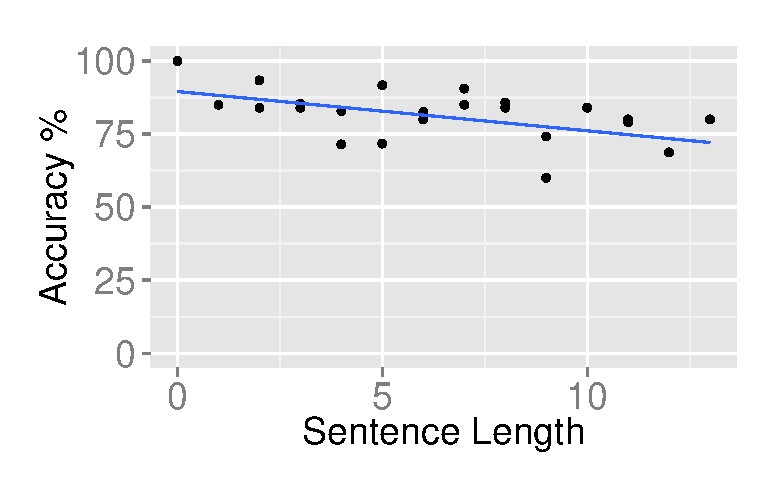
\includegraphics[width=1.0\linewidth]{2016_conll_verbpred/figures/full-pref-len}
 \caption{Full context set: Accuracy is generally high, but
   slightly decreases on longer, more complicated sentences, averaging
   81.1\%.}
 \label{fig:full_prefix}
  \end{center}
\end{figure}

In the {\bf random length set}, average accuracy over 200 sentences is 54.2\%,
significantly better than chance $(t(199) = 11.8205,
p<2.2\cdot10^{-16})$. Figure~\ref{fig:rand_prefix} shows the accuracy per
percentage of length of the presented sentence fragment.  A one-way \abr{anova}
reveals a significant effect of the sentence length
$(F(1,998)=57.44, p<7.94\cdot10^{-14})$.  We also find a significant effect of
the case density $(F(1,998)=5.884, p=0.0155)$.













\begin{figure}[t!]
 \begin{center}
 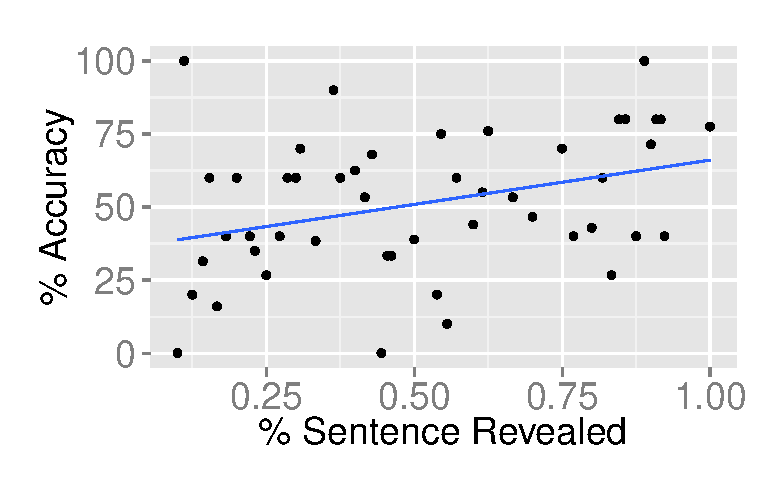
\includegraphics[width=1.0\linewidth]{2016_conll_verbpred/figures/rand-pref-len}
 \caption{Random length set: The accuracy of human verb predictions
   reliably increases as more of the sentence is revealed. }
 \label{fig:rand_prefix}
\end{center}
\end{figure}

\subsection{Discussion}

Predictability increases with the percent of the sentence available in all of
our experiments.  By the end of the sentence, the verb chunks are highly
predictable by humans in the multiple choice setting.  Participants choose the
final verb more accurately as they gain access to more case markers in the {\bf
  random length set} but not in the {\bf full context set}.

Case density is a significant factor in predictive accuracy on the
{\bf random length set} for humans, suggesting that case is more
helpful in predicting a sentence-final verb when the preceding
contextual information is insufficient. The following example
illustrates how case helps in prediction. The nominative and
accusative markers greatly narrow the choices, as shown in
(4).\footnote{A recent psycholinguistics study on incremental Japanese
  verb-final processing~\cite{momma2015timing} argues that native
  Japanese speakers plan verbs in advance, before the articulation of
  object nouns, but not subject nouns. Since case markers assign the
  roles of subject and object in Japanese, we expect that a high ratio
  of case markers to words will increase predictability of verbs. In
  addition, \newcite{yamashita1997effects} argues that the
  \textit{variety} of case markers increases predictability just
  before the verb.} Our results further support the proposition case
markers modulate predictability in \abr{sov} verb-final processing.
















































\begin{enumerate}[(4)]
 \setlength{\parskip}{-0.1cm}
 \item \label{quat-ex2}
  \gl{江戸幕府区-{\bf が}}{Edo shogunate-{\bf\abr{nom}}}
  \gl{成立すると}{establish-do-{\bf\abr{conj}}}
  \gl{寺院法度-{\bf に}-より}{temple-prohibition-etc.-\abr{acc}-for}
  \gl{---}{} \\
  `After Edo shogunate has established, due to the temple prohibition etc. ---'
\end{enumerate}






















In other cases, there exist choices, which, while incorrect, could naturally
complete the sentence.  These questions are frequently missed. For instance, in
one 90\% revealed sentence, the participant has the choices: (i) 収め
る (put-\abr{pres}), (ii) 厳しくなる (strict-become), (iii) {\it 収録されている}
(record-do.\abr{pass-aux.pres}), and (iv) 務める (work-\abr{pres}).  Choice (i)
is the correct answer, but choice (iii) is a reasonable choice for a Japanese
speaker.  All participants missed this question, and all chose the same wrong
answer (iii).  We leave a cloze task where participants can freely fill in the
sentence-final to future work.

These results provide a basis of comparison for automatic prediction.  In the
next section, we examine whether computational models can predict final
verbs and compare the models' performance to that of humans.


\section{Machine Verb Prediction}
\label{sec:language_model}

\begin{figure}[t!]
 \begin{center}
   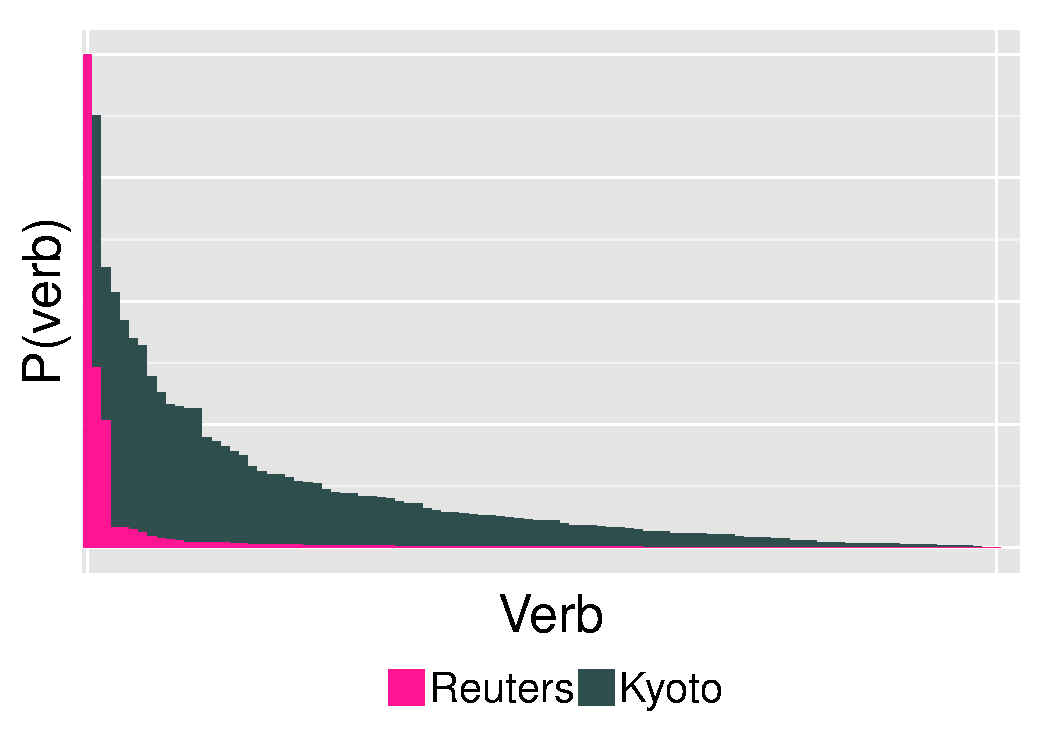
\includegraphics[width=1.0\linewidth]{2016_conll_verbpred/figures/top100verbs_kyoto_hist_no_suru-iru-aru-naru}
   \caption{Distribution of the top 100 content verbs in the Kyoto corpus and
     the Reuters Japanese news corpus.  Both are Zipfian, but the Reuters corpus
     is even more skewed, even with the common special cases
     excluded.}
 \label{fig:hist}
  \end{center}
\end{figure}

Now that we have the results of the previous section, we have
baselines against which we can compare computational verb prediction
approaches.  In this section, we introduce incremental verb
classification with a linear classifier.\footnote{While we use
  logistic regression, using hinge loss achieves similar accuracy.}
For our investigation of computational verb classification, we use two
very different languages that both have verb-final syntax---Japanese,
which is agglutinative, and German, which is not---and show that
discriminative classifiers can predict final verbs with increasing
accuracy as more context of sentences is revealed.

A simple verb prediction scheme applied to German~\cite{grissom2014}
achieves poor accuracy.  Their approach creates a Kneser-Ney \ngram{}
language model for the prior context associated with each verb in the
corpus; i.e., 50 $n$-gram models for 50 verbs. Given pre-verb $n$-gram
context $c$ in a sentence $S_t$, and verb prediction $v^{(t)}\in V$,
the verb selection is defined by the following equation:
\begin{equation}
  \label{eq:ngram}
  v^{(t)} \equiv \arg \max_v \prod_{c \in S_t} p(c \g v) p(v).
\end{equation}

It chooses the verb that maximizes the probability of the observed
context, scaled by the prior probability of the verb in the overall
corpus. Unsurprisingly, given the distribution of verbs in real data
(Figure~\ref{fig:hist}), this \ngram{}-based approach has low accuracy
and tends to predict the most common verb. For a translation system,
this often degenerates into the less interesting problem of whether to
trust whether the final verb is indeed a common one.  While this
improves translation delay, better predictions will lead to more
significant improvements.  We instead opt for a one-vs-all
discriminative classification approach.\footnote{One-vs-all
  classification builds a classifier for each class versus the
  aggregate all other classes.} 
\begin{figure}[t!]
  \begin{center} 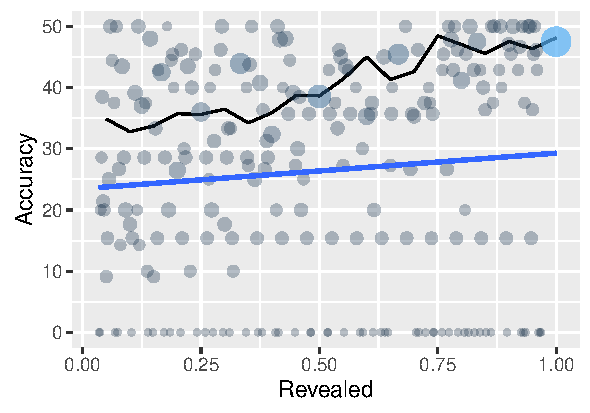
\includegraphics[width=1.0\linewidth]{2016_conll_verbpred/figures/CF_classify} \caption{Verb
      classification results on crowdsourced sentences. Despite many
      out-of-vocabulary items and significant noise, the average
      accuracy, shown in the non-monotonic line in the plot, increases
      over the course of the sentence. Larger, darker circles indicate
      more examples for a given position.  Accuracy was calculated by
      aggregating the guesses at 5\% intervals. }
\label{fig:CF_classify}
\end{center}
\end{figure}

\subsection{Classification on Human Data}
\label{sec:cf_classify}

We first incrementally classify verbs on the same 200 sentences from
Section~\ref{sec:human}.  Since the answer choices are often complex
verb \textit{bunsetsu} and since many of these verb phrase answer
choices do not appear among the most common verbs, lemmatizing the
verbs and performing one-vs-all classification yields extremely low
accuracy. Thus, we use binary classification with a single linear
classifier to produce a probability for each candidate answer,
encoding the verb phrase itself into the feature vector.

\subsubsection{Training a Morphological Model}
The processing is as follows: We train on 463,716 verb-final sentences
extracted from the training data.  We use both \textbf{context
  features} and \textbf{final verb features}.  Our context features,
i.e., those preceding the final verb, are represented as follows: the
context \textbf{unigrams} and \textbf{bigrams} take a value of $1$ if
they are present and $0$ otherwise; \textbf{case markers} observed in
the sentence context are represented as unigrams and bigrams in the
order that they appear; and we reserve a distinct feature for the
\textbf{last observed case marker} in the sentence.  Our \textbf{verb
  features} consist of the final verb's tokens given by the
morphological analyzer, which, in addition to the verb stem itself,
typically include tense and aspect information.  These are represented
as unigrams and bigrams in the feature vector.

To allow the classifier to learn, we must encode the interactions
between the verb features and the context features.  Thus, we
use the Cartesian product of sentence and verb features to encode
interactions between them: for each training sentence we generate
both a positive and a negative example. The example with the correct
verb phrase is labeled as a positive example ($+1$), and we uniformly
select a random verb phrase from one of the 500 most common verb
phrases and label it as negative ($-1$) example for the same sentence
context,\footnote{We experimented with several numbers of weighted
  negative examples and found that one negative example with of equal
  weight to the positive gave the best results of the configurations
  we tried.}  yielding 927,432 training examples and 267,037,571
features.


For clarity, we describe this feature representation more
formally. Given sentence $S_t$ with a pre-verb context consisting of
unigrams, bigrams, and case marker tokens, $C=\{c_0, ..., c_n\}$, and
\textit{bunsetsu} verb phrase tokens $A=\{a_0, ..., a_k\}$, the
feature vector consists of
$C\times A = \{c_0\wedge a_0, c_0\wedge a_1, ..., c_n\wedge a_k\}$,
where $\wedge$ concatenates the two context and answer strings.
During learning, the weights learned for the concatenated tokens are
thus based on the relationship between a context token and a
\textit{bunsetsu} token and mapped to $\{+1,-1\}$.  More concretely,
individual morphemes of the Japanese verb phrase are combined with the
pre-verb unigrams, bigrams, and uniquely identified case marker
tokens.  Accuracy improves when the morphemes used in the negative
examples and positive examples are disjoint; so, we enforce this
constraint when selecting negative examples. For example, if the
positive example includes the past tense morpheme, た, the negative
example is altogether disallowed from having this morpheme as a verb
feature.  
\subsubsection{Choosing an Answer}
At test time, we test progressively longer fragments of each sentence,
extracting the aforementioned features online until the entire
pre-verb context is available. For every sentence fragment, the
classifier determines the probability of each of the four possible
verbs by adding their verb features to the feature vector of the
example.  The answer choice with the highest probability of $+1$ (or
the lowest probability of $-1$) is chosen as the answer. By taking
this approach, we can model complex verbs and their context jointly.
Intuitively, the probability of a ($+1$) is the model's prediction of
how well the \textit{bunsetsu} verb phrase fits with the sentence
context (represented by the feature vector).

Some verbs are absent from the training data, forcing the classifier
to rely on morphemes to distinguish between them.  The
alternative---e.g., in a typical one-vs-all classification
approach---is that the classifier could reason from nothing whatsoever
when a fully-inflected verb is absent from the training data. Given
the complexity of \textit{bunsetsu}, this happens often even in large
corpora for a language such as Japanese.






\subsubsection{Multiple Choice Results}
Despite only choosing among four choices, this task is in many ways
more difficult than the 50-label classification problem described in
the next section because of the added complexity inherent modeling the
effect of morphemes and missing examples.  These limitations
notwithstanding, the accuracy does improve as more of the sentence is
revealed (Figure~\ref{fig:CF_classify}), indicating that the algorithm
learns to use these features to rank verbs, though the performance
significantly lags that of both the human participants and our later
experiments. 





Additionally, on the \textbf{full context set}, sentence length is
negatively correlated with accuracy
(Figure~\ref{fig:CF_classifier_length}), as in the much more
convincing results of our human experiments
(Figure~\ref{fig:full_prefix}), though the trend is not entirely
consistent, making it difficult to draw firm conclusions.  Case
density is again positively correlated with accuracy on both the
random (Figure~\ref{fig:CF_case_density}) and full context sets.
\begin{figure}[t!]
  \begin{center} 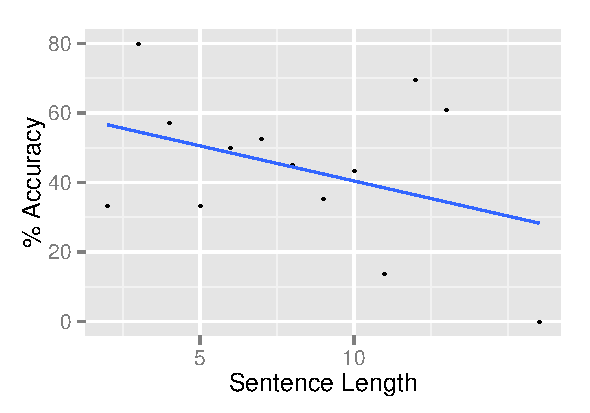
\includegraphics[width=1.0\linewidth]{2016_conll_verbpred/figures/CF_len_run2} \caption{
      Classification accuracy as a function of sentence length on the
      full context set. While there is a clear correlation between
      sentence length and accuracy, there are several
      outliers. Compare to Figure~\ref{fig:full_prefix}.}
\label{fig:CF_classifier_length}
\end{center}
\end{figure}

\paragraph{An Illustrative Example}

To gain some insight into how features can influence the classifier,
we here examine an example of the classifier's behavior on the
multiple choice data.

\begin{enumerate}[(5)]
\listsep
\item \label{sent-class}
\gl{少年時代-は}{childhood days-\abr{top}}
\gl{\hspace{2.5em}熊本藩-の}{Kumamoto domain-\abr{gen}}
\gl{藩校-で}{clan school-\abr{loc}}
\gl{儒学-を}{Confucianism-\abr{acc}}
\gl{学び、}{study:\abr{med}}
\gl{後-に}{subsequently-\abr{loc}}
\gl{西本願寺-において}{Nishihongan Temple-\abr{loc}}
\gl{修行-に}{discipline-\abr{all}}
\end{enumerate}
\begin{enumerate}[(6)]
\listsep
\item \label{sent-class-choices}
\begin{enumerate*}
  \item \gl{励ん-だ}{strive-PAST}
  \item \gl{創刊-さ-れ-る}{issue-do-PASS-NPST}
  \item \gl{加え-られ-てい-る}{add-PASS-CONT-NPST}
  \item \gl{勤め-る}{serve-NPST}
\end{enumerate*}
\end{enumerate}
In Example (5), the classifier incorrectly chooses ``issue'' as the
verb until observing the accusative case marker attached to
``Confucianism''.  At this point, the classifier's confidence in the
correct answer rises to 0.74---and correctly chooses ``strive''.  This
answer goes unchanged for the remainder of the sentence, though
``study'' attaches to ``Confucianism'', not the final verb. The
combined evidence, however, is enough for the classifier to select
correctly, and indeed, most of the following tokens only increase the
classifier's confidence.  Adding ``subsequently'' increases confidence
to 0.84, an intuitive increase given the likely tense information
contained in such a word.  The somewhat redundant case marker here
only increases confidence to 0.86.  Adding the reference to the temple
decreases confidence again to 0.79.  But adding the \textbf{final case
  marker}, which also forms a new bigram with the previous word,
results in a huge increase in confidence, to 0.90.

\subsection{Multiclass Verb Prediction}

\begin{figure}[t!]
  \begin{center} 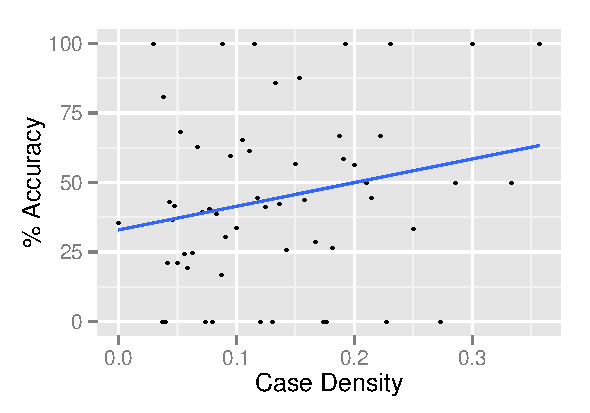
\includegraphics[width=1.0\linewidth]{2016_conll_verbpred/figures/CF_density_incremental} \caption{
      Classification accuracy as a function of case density on the
      incremental sentences.  The accuracy is correlated with case density,
      but the data are extremely noisy.  Full-context accuracy has a
      similar trend (not shown).}
\label{fig:CF_case_density}
\end{center}
\end{figure}

While the multiple choice experiment was more open-ended (predicting
random verbs), we now focus on a more constrained task: how well can
we predict the most frequent verbs.  This is the central conceit of
\newcite{grissom2014}: if you can do a good job of this, you can
improve simultaneous translation.  They show a slight improvement in
simultaneous translation by using \ngram{} language model-based verb
prediction.  We show a large improvement over their approach to verb
prediction using a discriminative multiclass logistic
classifier~\cite{langford2007vowpal}.

\paragraph{Data Preparation}

Our classes for multiclass classification are the fifty most common
verbs in the \abr{kft} (Japanese, as in the human study) and
Wortschatz corpora~\cite[German]{biemann2007leipzig}.

We use data from the training and test sets of the \abr{kft} Japanese
corpus of Wikipedia articles and a random split of the German
Wortschatz web corpus, from which we extract the verb-final
sentences. \newcite{grissom2014} use an \ngram{} model to distinguish
between the fifty most common German verbs for \abr{sov}-\abr{svo}
simultaneous machine translation, which we replicate as our baseline.
Following this study, we train a model on the fifty most common verbs
in the training set.

In Japanese, due to the small size of the standard test set, we
split the data randomly, training on 60,926 verb-final
sentences ending in the top fifty verbs and testing on 1,932.  Our total
feature count is 4,649,055.  We use the MeCab~\cite{kudo2005mecab}
morphological analyzer for segmentation and verb identification.  We
consider only verb-final sentences. We skip semantically vacuous
post-verbal copulas when identifying final verbs.

\paragraph{Finding Verbs}

We identify verbs in the German text with a part-of-speech
tagger~\cite{toutanova2003feature} and select from the top fifty
verbs.  We consider the sentence-ending set of verbs to be the final
verbs. We train on 76,209 verb-final sentences ending in the top fifty
verbs and test on 9,386.  In German, to approximate the case
information that we extract in Japanese, we test the inclusion of
equivalent unigram and bigram features for German \textbf{articles},
the surface forms of which determine the case of the next noun phrase.

In Japanese, we omit some special cases of light verbs that combine
with other verbs, as well as ambiguous surface forms and
copulas.\footnote{In Japanese, we omit some ambiguous cases and
  variants of ``is'' and ``do'': excluded are variants of
  \textit{suru} (``to do''), which combines with nouns to form new
  verbs, \textit{aru} (``is'', inanimate case), and \textit{iru}
  (``is'', animate case). The tokens \textit{aru} and \textit{iru}
  also combine with other verbs to change tense and aspect, in which
  case they are not verbs, and can form the copula \textit{de aru}.
  Distinguishing between all of these cases is beyond the scope of
  this study; so, they are excluded.  We also omit duplicates that are
  spelled differently (i.e., the same word but spelled without Chinese
  (\textit{kanji}) characters and slightly different forms of the same
  root).

  We also omit the light verb \textit{naru} (``to become'' or ``to
  make up'') for similar reasons to \textit{suru}.  The increasing
  trend shown in the results does not change with their inclusion.}

\paragraph{Features}

All features are encoded as binary features indicating their presence
or absence.  For Japanese, we again include \textbf{case unigrams},
and \textbf{case bigrams}, which encode as distinct features the for
case markers observed thus far.\footnote{For instance, given a
  sentence fragment X-に Y-を, representing X-\abr{dat} Y-\abr{acc},
  the case bigram would be に$\wedge$を.}  We also include a feature
for the \textbf{last observed case marker}.  For both Japanese and
German, we normalize the verbs to the non-past, plain form, both
providing more training data for each verb and simplifying the job of
our classifier.

German case is conveyed primarily through articles and pronouns, so we
include special features for articles.  For example, for the sentence
``Es wurde ihnen von einem alten Freund geholfen'', we add the
features \feat{\abr{art}\_es\_ihnen} and \feat{\abr{art}\_ihnen\_einem}
to convey case information beyond individual words and bigrams.

Individual tokens are also used as binary features, as well as token
bigrams.

\paragraph{An Example for Every Word}

In a simultaneous interpretation, a person or algorithm receives a
constant stream of words, and each new word provides new information
that can aid in prediction.  Previous predictive approaches to
simultaneous machine interpretation have taken this approach, and we
also use it here: as each new word is observed, we make a prediction.
This is a generalization of \emph{random} presentation of prefixes in
the human study.

\subsection{Classification Results and Discussion}

\paragraph{Better at the End}

A discriminative classifier does better than an \ngram{} classifier,
which has a tendency to over-predict frequent verbs.  By the end of
the sentence, accuracy reaches 39.9\% for German
(Figure~\ref{fig:german_unibi}) and 29.9\% Japanese
(Figure~\ref{fig:japanese_unibi}), greatly exceeding choosing the most
frequent class baseline of 3.7\% (German) and 6.05\% (Japanese).  The
\ngram{} language model also outperforms this baseline, but not by
much.  It also improves over the course of the sentence, but the model
cannot reliably predict more than a handful of verbs in either
language.


\begin{figure}[t!]
 \begin{center} 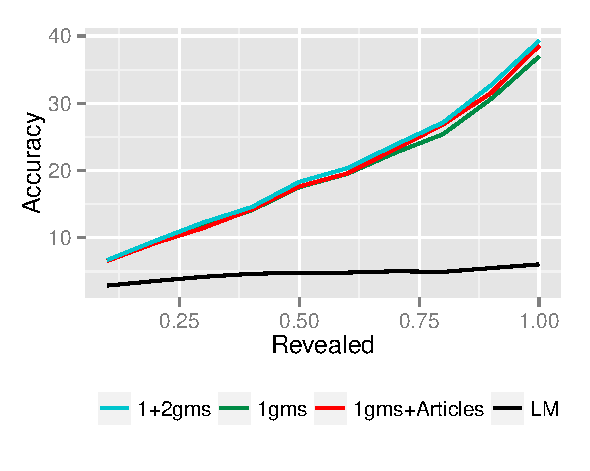
\includegraphics[width=1.0\linewidth]{2016_conll_verbpred/figures/german_top50_comparison}
\caption{German average prediction accuracy over the course of
  sentences. Bigrams help slightly in the second half of the sentence.
  Adding special features for case-assigning articles to unigrams
  nearly matches the performance of adding all bigrams in the final
  10\%. All handily outperform the trigram language
  model.}  \label{fig:german_unibi} \end{center}
\end{figure}

\paragraph{Richer Features Help (Mostly at the End)}

Bigram features help both languages, but Japanese more than German;
beyond bigrams, however, trigrams and longer features overfit the
training data and hurt performance.  The better performance for
Japanese bigrams is likely because word boundaries are not
well-defined in Japanese, and individual morphemes can combine in ways
that significantly add information.  German word boundaries are more
precise and words (particularly nouns) can carry substantial
information themselves.

Richer features matter more toward the end of the sentence.  In
Japanese, adding bigrams consistently outperforms unigrams alone, but
in both languages, adding special features for tokens with case
information helps almost as much as adding the full set of bigrams.
In Japanese, case markings always immediately follow the words marked,
and in German the articles precede the nouns to which they assign
case; thus, rather than relying on isolated unigrams, using bigrams
provides opportunities to encode case-marked words that more narrowly
select for verbs.  In Japanese, the differences are more pronounced
toward the very end of the sentences (and less so in German).


Richer features help more at the end, but not merely because the last
words of the sentence represent the densest feature vectors.  In
Japanese, the last word is usually a case-marked noun phrase or adverb
that matches the main predicate.  The final word is therefore immune
to subclause interference and must modify the final verb, boosting the
classifier performance in these final positions and amplifying the
predictive discrepancies between the various feature sets.  Accuracy
spikes at the end of Japanese sentences, where case information helps
nearly as much as adding the entire set of bigrams, further supporting
case information's importance.  Deeper processing---e.g., separating
case-marked words in subclauses from those in the main clause---would
likely be more useful.  Features and feature-selection strategies that
we tried which did not help included the following: adding only case
marker unigrams (instead of bigrams); filtering the features by using
only case-marked words; only allowing one word per case marker in the
feature vector (the most recent); using decaying weights on features
further in the past; adding part-of-speech tag $n$-grams; and adding
the word nearest to the centroid of the observed context in a word
embedding space.  While these features may have potential, they did
not lead to meaningful increases in accuracy in our experiments.

\begin{figure}[t!]
 \begin{center} 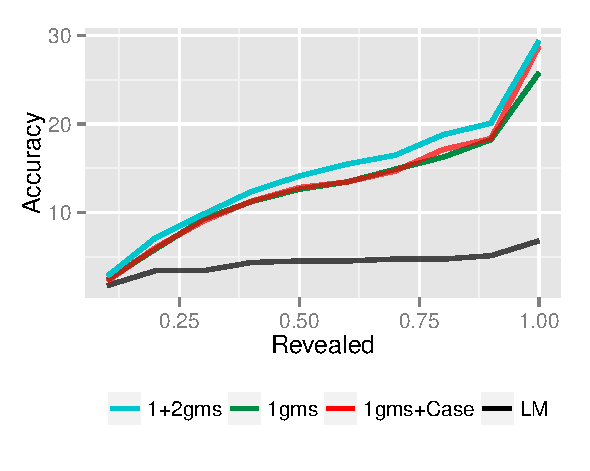
\includegraphics[width=1.0\linewidth]{2016_conll_verbpred/figures/japanese_top50_comparison_newsplit}
\caption{Japanese average prediction accuracy over the course of
  sentences. Adding bigrams consistently outperforms unigrams alone in
  Japanese, possibly due to the agglutinative nature of the language.
  The accuracies diverge the most toward the end of the sentences:
  Adding only explicit case markers to unigrams nearly matches
  performance of adding all bigrams toward the end. All outperform the
  trigram language model.}  \label{fig:japanese_unibi}
\end{center}
\end{figure}

\clearpage

\section{Related Work}
\label{sec:related}

While to our knowledge our work is the first in-depth study of
incremental verb prediction, it is not the first study of verb
prediction in humans or machines.  This section reviews that related
work.

\paragraph{Human Verb Prediction}

Prediction is easier with more context and explicit case markings.
\newcite{teramura-1987} shows that \emph{next word prediction} in
Japanese improves as more words are incrementally revealed.  While
only looking at verb prediction given the \emph{complete} preceding
context, \newcite{yamashita1997effects} finds that scrambling word
order in Japanese---a case rich language that allows such
scrambling---does not harm final verb prediction, but that explicit
case marking helps final verb prediction. Our results show that this
is true even for incremental verb
prediction. \newcite{levy2013expectation} also find that dative
markers aid German verb prediction.

Neurolinguistic measurements by \newcite{friederici2000verb} suggest
processing verb-final clauses in German use both semantic and
syntactic information, but that they are processed differently.  In
Japanese, \newcite{koso2011event} measure the effect of case markings
on predicting verbs with strong case preferences.  This is consistent
with our use of case-based features and suggests that further gains
are possible using richer syntactic
representations. \newcite{chow2015bag} use \abr{n400} measurements to
investigate two competing hypotheses for the initial prediction of an
upcoming verb: whether predictions are dependent on all words equally
(the Bag-of-words hypothesis), or alternatively, whether prediction is
selectively modulated by the final verb's arguments (the
Bag-of-arguments hypothesis).  They argue for the latter.

The literature on incremental verb prediction is sparse. A key finding
of \newcite{matsubara2002bilingual} is that Japanese-English simultaneous
interpreters, when given access to lecture slides, would refer to them
to predict the next phrase.

\paragraph{Prediction for Simultaneous Machine~Translation}

  The Verbmobil simultaneous translation
system~\cite{kay1992verbmobil} uses deleted
interpolation~\cite{jelinek1990self} to create a weighted $n$-gram
models to predict dialogue acts---almost identical to predicting the
next word~\cite{reithinger1996predicting}.
\newcite{konieczny2003anticipation} predict verbs with a recurrent
neural network, but \newcite{matsubara-00} was the first to use verb predictions
as part of a simultaneous interpretation system.  They use pattern
matching-based predictions of English verbs.  In contrast, \newcite{grissom2014}
use a statistical approach, using $n$-gram models to predict German verbs and
particles (in Section~\ref{sec:language_model} we show that this model predicts
verbs poorly).  However, their simultaneous translation system is able to learn
when to trust these predictions. \newcite{oda2015acl} extend the idea of using
prediction by predicting entire syntactic constituents for English-Japanese
simultaneous machine translation.  Both systems will likely benefit from our
improved verb prediction presented here.


\section{Conclusion}
\label{sec:conclusion}





Verb prediction is hard for both machines and humans but impossible
for neither.  Verbs become more predictable in discriminative settings
as more of the sentence is revealed, and when all of the prior context
is available, the verbs are highly predictable by humans when a
limited number of choices is available, though even then not perfectly
so.  While we make no claims concerning upper or lower bounds of
predictability in different settings, our dataset provides benchmarks
for future verb prediction research on publicly available corpora:
cognitive scientists can validate prediction, confusion, and
anticipation; engineers have a human benchmark for their systems; and
linguists can conduct future experiments on predictability.




Shallow features can be used to predict verbs more accurately with
more context. Improving verb prediction can benefit simultaneous
translations systems that have already shown to benefit from verb
predictions, as well as enable new applications that involve
predicting future linguistic input.

\section{Acknowledgments}
We would like to thank the anonymous reviewers for their comments.  We
thank Yusuke Miyao for his helpful support.  We would also like to
thank James H. Martin, Martha Palmer, Hal {Daum\'e III}, Mans Hulden,
Mohit Iyyer, John Morgan, Shota Momma, Graham Neubig, and Sho Hoshino
for their invaluable discussions and input.  This work was supported
by \abr{nsf} grant \abr{iis}-1320538.  Boyd-Graber is also partially
supported by \abr{nsf} grants \abr{ccf}-1409287 and
\abr{ncse}-1422492. Any opinions, findings, conclusions, or
recommendations expressed here are those of the authors and do not
necessarily reflect the view of the sponsor.

\end{CJK}
% include your own bib file like this:

\clearpage

\bibliographystyle{style/acl2016}
\bibliography{bib/journal-full,bib/jbg,bib/alvin,bib/alvin_prelims}
\end{document}
